
\cxset{style05/.style={
 name={Chapter},
 chapter color = magenta,
 chapter toc = true,
 numbering=arabic,
 number font-size=\Large,
 number font-family=\rmfamily,
 number font-weight=\normalfont\itshape,
 number color= purple,
 number before=\hspace*{-15pt},
 number dot=,
 number after=,
 number position=rightname,
 chapter font-family=sffamily,
 chapter font-weight= \bfseries\itshape,
 chapter font-size=\Large,
 chapter before={\hrule width \columnwidth \kern12.6pt \par\hfill},
 chapter after={\hfill\hfill\par},
 chapter color={magenta},
 chapter spaceout=none,
 title beforeskip={\vspace*{10pt}},
 title afterskip={\vspace*{30pt}\par},
 title before={\hfill},
 title after={\hfill\hfill \vskip12.6pt\hrule width \columnwidth \kern2.6pt },
 title font-family=\rmfamily,
 title font-color=black!90,
 title font-weight=\bfseries,
 title font-size=\huge,
 title font-shape = normal,
 header style= headings}}

\cxset{style05}
\chapter{Introduction to Style Five}\index{ch:style5}

\tcbset{width=\textwidth}
I think this style can be improved with a bit of color. You can experiment with it quite easily. The spacing on top of this style can also be adjusted to suit your typographical taste.
\medskip
\begin{figure}[ht]
\centering
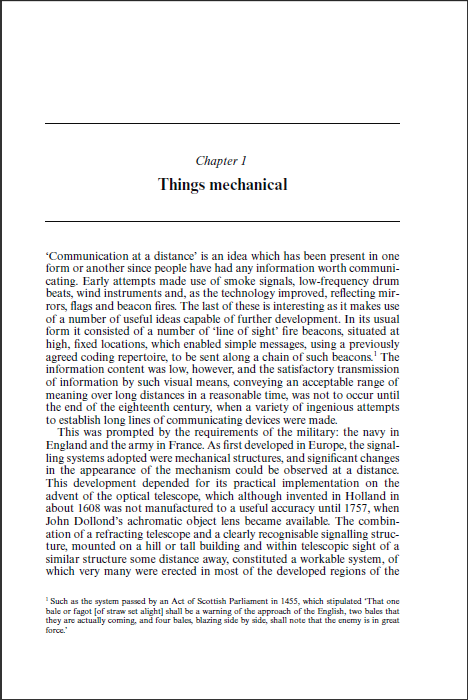
\includegraphics[width=0.6\textwidth]{./chapters/chapter05}
\end{figure}

%\section{General notes on rules}

LaTeX's default rules would normally give problems. Best is to use TeX's primitives to built them.

\index{rules!example color}

\begin{texexample}{}{}
\makeatletter
\hrule width 5cm \kern2.6\p@
AAAAAAAAAAAAAAAAAAAAA
\vskip2.6pt\hrule width 5cm
\medskip

Problem with LaTeX rules.

\rule{5cm}{0.4pt}\par
AAAAAAAAAAAAAAAAAAAAA\par%
\rule[6.5pt]{5cm}{0.4pt}

\def\rule{\@ifnextchar[\@rule{\@rule[\z@]}}
\def\@rule[#1]#2#3{%
 \leavevmode
 \hbox{%
 \setlength\@tempdima{#1}%
 \setlength\@tempdimb{#2}%
 \setlength\@tempdimc{#3}%
 \advance\@tempdimc\@tempdima%
 \vrule\@width\@tempdimb\@height\@tempdimc\@depth-\@tempdima}}

\def\thickrule{\leavevmode \leaders \hrule height 3pt \hfill \kern \z@}

{\color{teal}\hrule width 10.5cm height3pt \kern2.6\p@
    {{\color{black!80}\HUGE CHAPTER TITLE}}\vskip3pt
\hrule width 10.5cm height3pt}
\makeatother
\end{texexample}
